\documentclass[tikz]{standalone}

\usepackage{mathtools}
\usepackage{newtxtext,newtxmath}

%!TEX root = main.tex

% mytikzset
\usepackage{tikz}
\usetikzlibrary{positioning,arrows,shapes,patterns}
\usetikzlibrary{decorations.pathmorphing}
\usetikzlibrary{decorations.markings}
\usetikzlibrary{decorations.pathreplacing}
\usetikzlibrary{calc}
\usetikzlibrary{patterns}
\usetikzlibrary{decorations.markings}
\usetikzlibrary{petri}

\tikzset{
  vector/.style={thick,double,draw=black, postaction={decorate},
    decoration={markings,mark=at position .6 with {\arrow[black,scale=0.4]{triangle 45}}}},
  axial/.style={thick,double,densely dashed,draw=black, postaction={decorate},
    decoration={markings,mark=at position .6 with {\arrow[black,scale=0.4]{triangle 45}}}},
  gluon/.style={decorate, draw=black,
    decoration={coil,aspect=0.3,segment length=5pt,amplitude=3pt}},
  pseudo/.style={thick, dashed, draw=black, postaction={decorate},
    decoration={markings,mark=at position .6 with {\arrow[red,scale=0.5]{triangle 45}}}},
  scalar/.style={thick,draw=black, postaction={decorate},
    decoration={markings,mark=at position .6 with {\arrow[black,scale=0.5]{triangle 45}}}},
  cut/.style={draw=black, decorate, decoration={snake, segment length=1mm, amplitude=0.2mm}}
}


\begin{document}
\nopagecolor
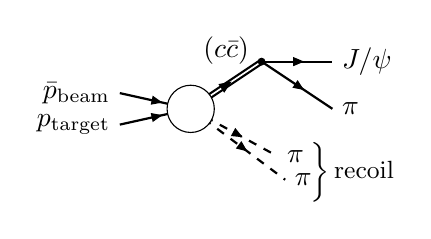
\begin{tikzpicture}[node distance=0.6cm and 0.9cm,baseline=1cm]
  % \coordinate[] (a2);
  % \coordinate[] (z2);
  \coordinate[] (b2);
  \coordinate[left=of b2,label=left:$\bar{p}_\text{beam}$, yshift=2mm] (b1);
  \coordinate[left=of b2,label=left:$p_\text{target}$, yshift=-2mm] (j1);
  \coordinate[above right=of b2] (b4);
  \coordinate[below right=of b2,xshift=2mm,label=right:$\pi$] (b5);
  \coordinate[below right=of b2,xshift=3mm,yshift=-3mm,label=right:$\pi$] (j5);
  \coordinate[right=of b4,label=right:$J/\psi$] (c1);
  \coordinate[below right=of b4,label=right:$\pi$] (c2);

  % \draw[scalar]  (b2) -- node[label=left:{$\mathbb{P}$}] {} (a2);
  \draw[scalar]  (b1) -- (b2);
  \draw[scalar]  (j1) -- (b2);
  \draw[scalar, dashed]  (b2) -- (b5);
  \draw[scalar, dashed]  (b2) -- (j5);
  \draw[vector]  (b2) -- node[label=above:{$(c\bar{c})$}] {} (b4);
  \draw[scalar]  (b4) -- (c1);
  \draw[scalar]  (b4) -- (c2);

  \node[right=of j5,xshift=-7mm,yshift=1mm] {\small \bigg\}\,recoil};
  \draw[fill=white] (b2) circle [radius=0.3];
  \fill[black] (b4) circle [radius=0.05];
\end{tikzpicture}
\end{document}
